\documentclass{mipt-thesis-ms}
% Следующие две строки нужны только для biblatex. Для inline-библиографии их следует убрать.
\usepackage{mipt-thesis-biblatex}
\usepackage{biblatex}
\addbibresource{Diplom.bib}
\usepackage{hyperref}
\usepackage{graphicx}
\usepackage{makecell}
\DeclareGraphicsExtensions{.pdf,.png,.jpg}

\title{Одновременное картирование и локализация по видео с построением плотной карты в реальном времени}
\author{Муравьев К.\,Ф.}
%\supervisor{Яковлев К.\,С.}
%\groupnum{М05-914Б}
%\faculty{Физтех-школа прикладной математики и информатики}
%\department{Кафедра анализа данных}

\begin{document}
	%\frontmatter
	%\maketitle
	%\titlecontents
	%\mainmatter
	
	%----------------------------------------------------------------------------------------------------------------------------
	% INTRODUCTION
	%----------------------------------------------------------------------------------------------------------------------------
	
	\chapter{Введение}
	
	Введение.
	
	%----------------------------------------------------------------------------------------------------------------------------
	% PROBLEM SETTING
	%----------------------------------------------------------------------------------------------------------------------------
	
	\chapter{Постановка задачи одновременного картирования и локализации}
	
	\section{Одновременное картирование и локализация по видеопотоку (vSLAM)}
	
	Задача одновременного картирования и локализации по визуальным данным (visual-based simultaneous localization and mapping, vSLAM) возникает при навигации в неизвестной среде робота, не имеющего на борту никаких сенсоров, кроме единственной видеокамеры. Задача формулируется следующим образом: по изображениям с видеокамеры необходимо построить трёхмерную модель окружающего пространства, и определить траекторию перемещения камеры в этом пространстве.
	
	Математически задачу можно сформулировать таким образом: существует набор точек в трёхмерном пространстве $\{M_i \} = \textbf{W}, M_i \in \mathbb{R}^3$, называемый сценой. Дана последовательность кадров $\{\mathcal{P}^t\}$. Каждый кадр является проекцией точек сцены с ракурса $\mathcal{R}_t = (x_t, y_t, z_t, p_t, r_t, w_t) \in \mathbb{R}^6$. Числа $x_t, y_t, z_t$ задают пространственное положение камеры в момент времени $t$, а $p_t, r_t, w_t$ - углы направления главной оптической оси камеры в момент времени $t$.
	
	Кадр представляется в виде трех матриц размер $H \times W$, содержащих числа от 0 до 1 - яркости соответствующих пикселей красной, синей и зеленой цветовых компонент:
	$$\mathcal{P}^t = \{\mathcal{P}^t_{c,h,w}\}_{c \in [1 \dots 3], h \in [1 \dots H], w \in [1 \dots W]} \in [0, 1]^{3 \times H \times W}$$
	Каждый элемент $c$-й матрицы кадра $\mathcal{P}^t_{c,h,w}$ представляет собой яркость $c$-й цветовой компоненты точки, которая в момент времени $t$ спроецировалась на позицию $(h, w)$ в матрице камеры:
	$$P(\mathcal{R}_t, M_i) = (h, w) \Rightarrow \mathcal{P}^t_{c,h,w} = I_c(\mathcal{R}_t, M_i),$$
	где $P(\mathcal{R}_t, M_i): \mathbb{R}^6 \times \mathbb{R}^3 \rightarrow \mathbb{R}^2$ - функция проекции точки пространства на матрицу камеры, принимающая на вход ракурс и положение точки в пространстве и возвращающая координаты проекции, а $I_c (\mathcal{R}_t, M_i): \mathbb{R}^6 \times \mathbb{R}^3 \rightarrow [0, 1]$ - функция яркости $c$-й цветовой компоненты точки $M_i$, рассматриваемой с ракурса $\mathcal{R}_t$.
	
	По имеющейся последовательности кадров $\{\mathcal{P}_t\}$ необходимо найти $(x_t, y_t, z_t)$ для всех моментов времени $t$ - координаты ракурсов $\mathcal{R}_t$, а также как можно большее количество координат точек $M_i$.
	
	\section{Одновременное картирование и локализация по видеоданным с картами глубины (RGBD-SLAM)}
	
	Задача одновременного картирования и локализации по видеоданным и данным глубины (RGBD-SLAM) возникает при навигации в неизвестной среде робота, имеющего на борту видеокамеру и сенсор глубины. Задача формулируется следующим образом: по изображениям с видеокамеры и картам глубины этих изображений необходимо построить трёхмерную модель окружающего пространства, и определить траекторию перемещения камеры в этом пространстве.
	
	Математически задачу можно сформулировать таким образом: существует набор точек в трёхмерном пространстве $\{M_i \} = \textbf{W}, M_i \in \mathbb{R}^3$, называемый сценой. Дана последовательность кадров $\{\mathcal{P}^t\}$ и карт глубины $\{\mathcal{D}^t\}$.
	
	Кадр представляется в виде трех матриц размер $H \times W$, содержащих числа от 0 до 1 - яркости соответствующих пикселей красной, синей и зеленой цветовых компонент:
	$$\mathcal{P}^t = \{\mathcal{P}^t_{c,h,w}\}_{c \in [1 \dots 3], h \in [1 \dots H], w \in [1 \dots W]} \in [0, 1]^{3 \times H \times W}$$
	Каждый элемент $c$-й матрицы кадра $\mathcal{P}^t_{c,h,w}$ представляет собой яркость $c$-й цветовой компоненты точки, которая в момент времени $t$ спроецировалась на позицию $(h, w)$ в матрице камеры:
	$$P(\mathcal{R}_t, M_i) = (h, w) \Rightarrow \mathcal{P}^t_{c,h,w} = I_c(\mathcal{R}_t, M_i)$$
	Карта глубины представляется в виде матрицы размера $H \times W$, содержащей положительные действительные числа - глубины соответствующих пикселей:
	$$\mathcal{D}^t = \{\mathcal{D}^t_{h,w}\}_{h \in [0 \dots H], w \in [0 \dots W]}$$
	Элемент матрицы карты глубины $D^t_{h,w}$ представляет собой расстояние от положения камеры в момент времени $t$ до точки, которая в момент времени $t$ спроецировалась на позицию $(h, w)$ в матрице камеры: 
	$$P(\mathcal{R}_t, M_i) = (h, w) \Rightarrow \mathcal{D}^t_{h,w} = \rho(M_i, (x_t, y_t, z_t))$$
	Здесь $P(\mathcal{R}_t, M_i): \mathbb{R}^6 \times \mathbb{R}^3 \rightarrow \mathbb{R}^2$ - функция проекции точки пространства на матрицу камеры, принимающая на вход ракурс и положение точки в пространстве и возвращающая координаты проекции, а $I_c (\mathcal{R}_t, M_i): \mathbb{R}^6 \times \mathbb{R}^3 \rightarrow [0, 1]$ - функция яркости $c$-й цветовой компоненты точки $M_i$, рассматриваемой с ракурса $\mathcal{R}_t$. Функция $\rho: \mathbb{R}^3 \times \mathbb{R}^3 \rightarrow \mathbb{R}_{+}$ задает евклидово расстояние между двумя точками в пространстве.
	
	По имеющейся последовательности кадров $\{\mathcal{P}_t\}$ и карт глубин $\{\mathcal{D}_t\}$ необходимо найти $(x_t, y_t, z_t)$ для всех моментов времени $t$ - координаты ракурсов $\mathcal{R}_t$, а также как можно большее количество координат точек $M_i$.
	
	\section{Сведение RGBD-SLAM к vSLAM: восстановление карт глубин по видеопотоку}
	
	Задача восстановления карт глубин по видеопотоку возникает при навигации в неизвестной среде робота, не имеющего на борту никаких сенсоров, кроме видеокамеры. С помощью восстановления глубины по видеопотоку можно свести задачу vSLAM к задаче RGBD-SLAM, для которой разработаны более эффективные методы решения.
	
	Задача восстановления карт глубин по видеопотоку формулируется следующим образом: по изображениям, поступающим с единственной видеокамеры, необходимо определить расстояния до всех объектов, изображенных на этих изображениях. Математически задачу можно сформулировать таким образом: существует набор точек в трёхмерном пространстве $\{M_i \} = \textbf{W}, M_i \in \mathbb{R}^3$, называемый сценой. Дана последовательность кадров $\{\mathcal{P}^t\}$. Каждый кадр является проекцией точек сцены с ракурса $\mathcal{R}_t = (x_t, y_t, z_t, p_t, r_t, w_t) \in \mathbb{R}^6$. Числа $x_t, y_t, z_t$ задают пространственное положение камеры в момент времени $t$, а $p_t, r_t, w_t$ - углы направления главной оптической оси камеры в момент времени $t$.
	
	Кадр представляется в виде трех матриц размер $H \times W$, содержащих числа от 0 до 1 - яркости соответствующих пикселей красной, синей и зеленой цветовых компонент:
	$$\mathcal{P}^t = \{\mathcal{P}^t_{c,h,w}\}_{c \in [1 \dots 3], h \in [1 \dots H], w \in [1 \dots W]} \in [0, 1]^{3 \times H \times W}$$
	Каждый элемент $c$-й матрицы кадра $\mathcal{P}^t_{c,h,w}$ представляет собой яркость $c$-й цветовой компоненты точки, которая в момент времени $t$ спроецировалась на позицию $(h, w)$ в матрице камеры:
	$$P(\mathcal{R}_t, M_i) = (h, w) \Rightarrow \mathcal{P}^t_{c,h,w} = I_c(\mathcal{R}_t, M_i),$$
	где $P(\mathcal{R}_t, M_i): \mathbb{R}^6 \times \mathbb{R}^3 \rightarrow \mathbb{R}^2$ - функция проекции точки пространства на матрицу камеры, принимающая на вход ракурс и положение точки в пространстве и возвращающая координаты проекции, а $I_c (\mathcal{R}_t, M_i): \mathbb{R}^6 \times \mathbb{R}^3 \rightarrow [0, 1]$ - функция яркости $c$-й цветовой компоненты точки $M_i$, рассматриваемой с ракурса $\mathcal{R}_t$.
	
	По имеющейся последовательности кадров $\{\mathcal{P}_t\}$ необходимо для всех $h,w,t$ найти $\mathcal{D}^t_{h,w}$ - расстояния от положения камеры в момент $t$ до точек сцены, изображенных на кадре:
	$$P(\mathcal{R}_t, M_i) = (h, w) \Rightarrow \mathcal{D}^t_{h,w} = \rho((x_t, y_t, z_t), M_i)$$
	
	%----------------------------------------------------------------------------------------------------------------------
	% EVALUATION
	%-----------------------------------------------------------------------------------------------------------------------
		
	\chapter{Оценка качества одновременного картирования и локализации}
	
	\section{Метрики качества}
	
	Для оценки качества алгоритмов одновременного картирования и локализации (vSLAM) и их сравнения между собой необходимо выбрать метрику оценки качества. Алгоритмы vSLAM, как правило, дают в качестве выходных данных карту окружающей местности и траекторию перемещения камеры. Поэтому для оценки качества vSLAM существуют две группы метрик - метрики качества локализации и метрики качества картирования.
	
	\subsection{Метрики качества локализации}
	
	Метрики качества локализации, как правило, сравнивают траекторию, вычисленную алгоритмом SLAM, с истинной траекторией. Траектория представляет собой набор поз, каждая из которых включает трехмерную позицию (положение камеры в пространстве) и трехмерную ориентацию (направление главной оптической оси камеры). Оценка качества локализации сводится к вычислению ошибки между набором истинных и предсказанных поз. В научной литературе используются абсолютные и относительные ошибки, а также ошибки смещения и поворота.
	
	Обозначим истинную траекторию как $\{(p_t, q_t)\}, t \in \{1, \dots, T\}$, где $p_t \in \mathbb{R}^3$ - трехмерная позиция камеры в момент времени $t$, $q_t \in \mathbb{R}^3$ - вектор направления главной оптической оси камеры в момент времени $t$. Предсказанную траекторию обозначим как $\{(\widehat{p_t}, \widehat{q_t})\}, t \in \{1, \dots, T\}$.
	
	Одной из наиболее распространенных метрик является абсолютная ошибка траектории (Absolute Trajectory Error, ATE). Она формулируется как среднеквадратичное отклонение точек предсказанной траектории от истинной:
	
	\begin{equation}
	\label{eq_ate}
	ATE = \sqrt{\frac{1}{T} \sum_{t=1}^T || p_t - \widehat{p_t} ||_2^2}
	\end{equation}
	
	Помимо абсолютной ошибки траектории, также широко применяется относительная ошибка позы (Relative Pose Error, RPE). Она формулируется как среднеквадратичное отклонение предсказанного смещения на каждом шаге от истинного:
	
	$$\Delta p_t = M_{q_{t-1}}^{-1} (p_t - p_{t-1});\ \Delta \widehat{p_t} = M_{\widehat{q_{t-1}}}^{-1} (\widehat{p_t} - \widehat{p_{t-1}})$$
	
	\begin{equation}
	\label{eq_rpe}
	RPE = \sqrt{\frac{1}{T} \sum_{t=1}^T ||\Delta p_t - \Delta \widehat{p_t} ||_2^2},
	\end{equation}
	
	где $M_{q_{t-1}}, M_{\widehat{q_{t-1}}}$ - матрицы вращения, переводящие вектор (1, 0, 0) в векторы $q_{t-1}$ и $\widehat{q_{t-1}}$ соответственно.
	
	\textbf{TODO:} Поясняющая картинка!
	
	В работе \cite{geiger2012we} приводятся следующие метрики качества локализации: относительное смещение и относительная ошибка поворота. Данные метрики учитывают не только расхождение между траекториями, но и их длину:
	
	\begin{equation}
	\label{eq_etrans}
	E_{trans} = \frac{1}{T} \sum\limits_{t=1}^T \frac{|| M_{q_{t-1}} (p_t - p_{t-1}) - M_{\widehat{q_{t-1}}} (\widehat{p_t} - \widehat{p_{t-1}}) ||_2}{|| p_t - p_{t-1} ||_2}
	\end{equation}
	
	\begin{equation}
	\label{eq_erot}
	E_{rot} = \frac{1}{T} \frac{\angle(M_{q_{t-1}} (p_t - p_{t-1}), M_{\widehat{q_{t-1}}} (\widehat{p_t} - \widehat{p_{t-1}}))}{|| p_t - p_{t-1} ||_2}
	\end{equation}
	
	\subsection{Метрики качества картирования}
	
	Оценка качества картирования является более сложной задачей, чем оценка качества локализации. Если при оценке качества локализации легко установить соответствия между точками истинной и предсказанной траекторий (по времени прохождения данных точек), то однозначного соответствия между точками истинной и предсказанной карты не существует. Как правило, соответствия устанавливаются методом ближайшего соседа - каждая точка предсказанной карты сопоставляется с ближайшей к ней точкой истинной карты. Такой подход применяется в программном пакете CloudCompare\footnote{http://cloudcompare.org/} и в работах \cite{handa2014benchmark}\cite{wasenmuller2016corbs}. Применяя среднеквадратичную ошибку (RMSE) в этом подходе, получаем абсолютную ошибку картирования (Absolute Mapping Error, AME).
	
	По заданной истинной карте, представленной в виде трехмерного облака точек:
	
	\begin{equation}
	M=\{m_i \in \mathbb{R}^3; i \in [1;n]; n \in \mathbb{N}\}
	\label{eq_vslam_map}
	\end{equation}
	
	и карте, построенной алгоритмом vSLAM:
	
	\begin{equation}
	M^*=\{m^*_j \in \mathbb{R}^3; j \in [1;N]; n \in \mathbb{N}\}
	\label{eq_gt_map}
	\end{equation}
	
	абсолютная ошибка картирования вычисляется следующим образом:
	
	$$j' = \arg\min\limits_{i} ||m^*_j - m_{i}||_2$$
	
	\begin{equation}
		\label{eq_ame}		
		AME(M, M^*) = \sqrt{\frac{1}{N} \sum\limits_{j=1}^N ||m^*_j  - m_{j'}||_2^2}
	\end{equation}
	
	Однако существуют ситуации, когда абсолютная ошибка картирования, вычисленная по методу ближайшего соседа, не является репрезентативной. Например, при картировании помещений большой площади точки стен предсказанной карты могут быть сопоставлены с точками пола истинной карты. Таким образом абсолютная ошибка картирования может быть небольшой даже при неточном картировании. Так получилось в одном из экспериментов, описанных в разделе \ref{section_experiments}. При картировании помещений алгоритмом SLAM с глубинами, предсказанными нейросетью, обнаружилось, что карты визуально получались довольно неточные, при этом значение метрики AME на этих картах оказалось низким. При удалении точек пола из истинных и предсказанных карт значение метрики AME существенно выросло (см. рис. \ref{figure_floor}). Таким образом, в контексте оценки качества алгоритмов vSLAM метрика AME с сопоставлением по методу ближайшего соседа малоприменима.
	
	В рамках данной работы был разработан новый способ сопоставления точек истинной и предсказанной карты, учитывающий контекст задачи визуального картирования и локализации и основанный на сопоставлении ракурсов, с которых видны точки истинной и предсказанной карт. Ниже приведено подробное описание разработанного метода.
	
	\begin{figure}
		%\centering
		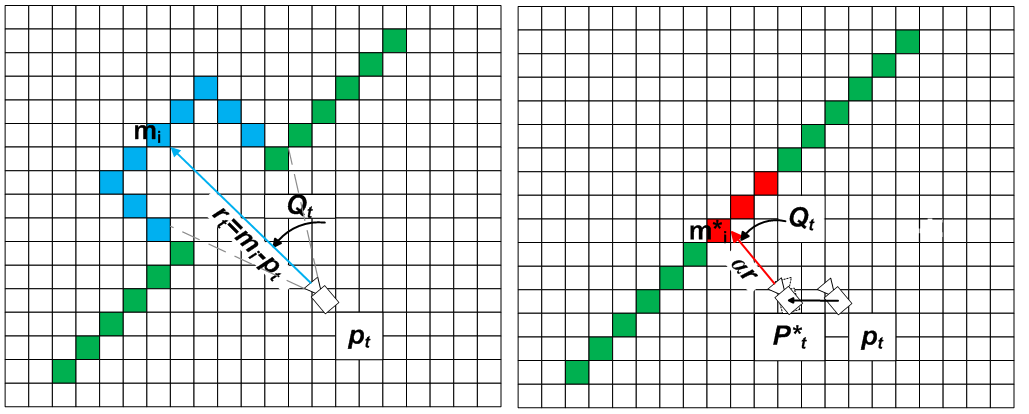
\includegraphics[width=1.0\textwidth]{img/corresp.png}
		\caption{Пример сопоставления точек истинной и предсказанной карты с использованием ракурса}
		\label{figure_correspondences}
	\end{figure}
	
	Пусть $M,\ M^*$ - истинная и построенная алгоритмом vSLAM карты (\ref{eq_gt_map}, \ref{eq_vslam_map}); $m_i^*$ - точка карты $M^*$, попадающая в поле зрения камеры в момент времени $t$; $p_t^*, q_t^*$ - предсказанные методом vSLAM положение и ориентация камеры в момент времени $t$; $p_t, q_t$ - истинные положение и ориентация камеры в момент $t$. Нужно построить функцию $f: M^* \longrightarrow M$, устанавливающую соответствие между точками построенной и истинной карты.
	
	Обозначим матрицы вращения, заданные ориентациями $q_t$ и $q_t^*$, как $M_{q_t}$ и $M_{q_t^*}$ соответственно. Вектор $r_t = (M_{q_t^*})^{-1} M_{q_t} (m_i^* - p_t)$ соответствует направлению с позиции камеры на точку $m_i^*$ в истинной карте (точка $p_t + \alpha r_t$ в истинной карте будет видна в момент $t$ под тем же ракурсом, что точка $m_i^*$ в предсказанной карте, см. рис. \ref{figure_correspondences}). Точке $m_i^*$ будет сопоставлена ближайшая точка истинной карты, которая видна под таким ракурсом:
	
	\begin{equation}
	\label{eq_corresp_function}
	f(m_i^*) = p_t + \alpha r_t;\ \ \alpha = \arg\min \limits_{\alpha'}: p_t + \alpha' r_t \in M
	\end{equation}
	
	\begin{figure}
		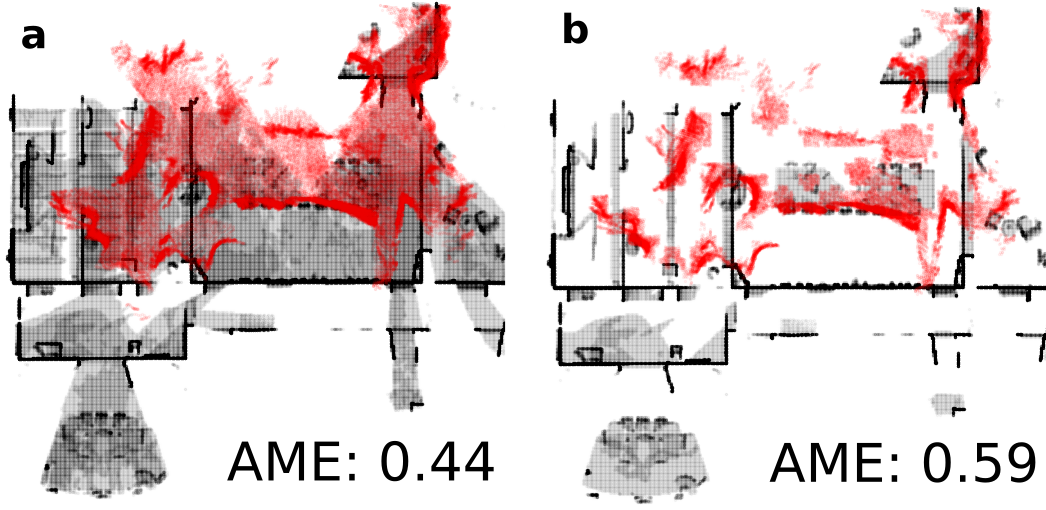
\includegraphics[width=1.0\textwidth]{img/1_first_paired.png}
		\caption{Исходные карты (a) и карты с вырезанным полом (b). Черным отмечены точки истинной карты, красным - предсказанной методом vSLAM карты. Метрика AME на картах с полом значительно ниже, чем на тех же картах без пола.}
		\label{figure_floor}
	\end{figure}

	Абсолютная и относительная ошибки картирования с таким методом сопоставления будет выглядеть следующим образом:
	
	\begin{equation}
		\label{eq_ame_our}
		AME(M, M^*) = \sqrt{\frac{1}{N} \sum\limits_{i=1}^N ||m_i^* - f(m_i^*)||_2^2}
	\end{equation}
	
	\begin{equation}
	\label{eq_rme_our}
	RME(M, M^*) = \sqrt{
	\begin{aligned}
	\frac{1}{N} \sum\limits_{i=1}^N ||M_{q_t^*}^{-1}(m_i^* - p_t^*) - \\
		- M_{q_t}^{-1} (f(m_i^*) - p_t)||_2^2
	\end{aligned}
	}
	\end{equation}
	
	При использовании данных метрик возникает следующая проблема. Одна точка карты может быть видна с разных позиций (т.е. для одной точки $m_i^*$ есть несколько $t$, по которым можно построить разные соответствия). Поэтому нужно определиться со способом выбора $t$. В данной работе были рассмотрены следующие варианты:
	
	\begin{itemize}
		\item $t$ выбирается как момент, в который точка $m_i^*$ попала в поле зрения камеры в первый раз;
		\item $t$ выбирается как момент, в который точка $m_i^*$ попала в поле зрения камеры в последний раз;
		\item $t$ выбирается как момент видимости точки $m_i^*$, в который точка была наиболее близка к позиции камеры;
		\item $t$ рассматриваются все моменты $t$, в который точка попадала в поле зрения камеры; при вычислении метрики берется усредненное расстояние между точкой $m_i^*$ и точками $f(m_i^*, t)$ для всех $t$.
	\end{itemize}

	Последний вариант выбора $t$ приводит к большим вычислительным затратам, однако метрика с ним получается наиболее стабильной. Для оценки качества алгоритмов vSLAM в данной работе был выбран именно этот вариант.
	
	Метрики AME и RME, вычисленные на основе функции сопоставления $f$, являются более подходящими для оценки качества алгоритмов vSLAM, поскольку они учитывают не только расстояния между точками, но и процесс построения карты алгоритмом vSLAM. Также данные метрики являются более устойчивыми к различным изменениям структуры карты (например, удаление точек пола), что подтверждено экспериментами, описанными в разделе \ref{section_experiments}.
	
	\section{Коллекции данных}
	
	 Проведение натурных экспериментов на реальной робототехнической системе затратно, а повторяемость таких экспериментов затруднена, поэтому для тестирования алгоритмов vSLAM и их сравнения между собой обычно применяются предварительно собранные коллекции данных. Такие коллекции должны включать в себя запись видеопотока с камеры робота (в случае RGB-D камеры - запись изображений и данных о глубине), а также данные об истинных позициях робота и истинной карте окружающей местности для вычисления метрик качества. Подобные коллекции бывают двух видов: собранные в реальном мире и синтетические.
	 
	 При сборке коллекций данных в реальном мире возникают сложности с определением истинной траектории робота и точной модели окружающей местности. Для вычисления точных данных о движении робота и его окружающей среде необходимо редкое и дорогостоящее оборудование, а также значительные временные затраты. Как правило, в коллекциях данных из реального мира имеются данные лишь о траектории робота, собранные с помощью систем отслеживания движения (Motion-capture System \cite{kurihara2002optical}), а истинные карты окружающей среды отсутствуют. При тестировании методов vSLAM на таких коллекциях можно вычислить метрики ATE \ref{eq_ate}, RPE \ref{eq_rpe}, $E_{trans}$ \ref{eq_etrans}, $E_{rot}$ \ref{eq_erot}, но невозможно вычислить метрики AME и RME (\ref{eq_ame}, \ref{eq_ame_our}, \ref{eq_rme_our}).
	 
	 Синтетические коллекции данных, а также различные робототехнические симуляторы (например, \cite{koenig2004design} \cite{rooban2021coppeliasim}) позволяют легко получить истинные карты и траектории, однако в большинстве обладают низкой фотореалистичностью, что критически важно для алгоритмов визуального картирования и локализации.
	
	\subsection{Коллекции данных из реального мира}
	
	Коллекции данных, собранные с помощью прогонов системы, оснащенной камерой, по некоторой траектории в реальном мире, на данный момент очень широко распространены. Имеется множество коллекций, в которых представлены прогоны робота в помещениях, а также несколько крупных коллекций, собранных с автомобиля, оснащенного большим количеством датчиков. В большинстве таких коллекций представлены истинные траектории движения робота, но отсутствуют истинные карты окружающей местности. Подобные датасеты хорошо подходят для оценки качества локализации методов vSLAM, однако оценка качества картирования на них затруднена или вовсе невозможна. Ниже представлен обзор наиболее известных наборов данных из реального мира для тестирования vSLAM.
	
	Одним из самых известных датасетов для тестирования алгоритмов SLAM является KITTI \cite{geiger2012we}. Он содержит 22 сцены, записанные с автомобиля в городской среде. Общая длина проезда составляет 39 км. Датасет содержит порядка 41 тысячи кадров видеопотока, записанного со стереокамеры, а также данные трехмерного лазерного сканера (лидара) и инерциальной навигационной системы (ИНС) совместно с показаниями GPS. В данной коллекции также представлены истинные позиции, собранные с помощью агрегации данных GPS и ИНС, а также качественной пост-обработки. Истинная карта окружающих объектов не представлена, однако она может быть приблизительно воссоздана по истинным позициям автомобиля и облакам точек с лидара.
	
	Помимо исходных данных с сенсоров, в KITTI также представлено программное обеспечение, необходимое для вычисления метрик качества локализации. Также в датасете предоставлены данные для тестирования некоторых других методов компьютерного зрения: семантической сегментации, детекции объектов, вычисления оптического потока. Данный датасет широко используется для оценки качества методов визуальной одометрии \cite{geiger2015kitti}, а также для обучения различных нейросетевых моделей \cite{li2018megadepth} \cite{zhou2017unsupervised} \cite{patil2020don}. Однако оценка качества картирования на данном датасете затруднительна, поскольку истинных карт окружающей среды в датасете не предоставлено.
	
	
	
	\subsection{Коллекции синтетических данных}
	
	Тут про симуляторы, Scannet и наш MAOMaps.
	
	%------------------------------------------------------------------------------------------------------------------------
	% METHODS
	%------------------------------------------------------------------------------------------------------------------------
	
	\chapter{Методы решения задачи vSLAM}
	
	\section{Классические методы}
	
	\subsection{ORB-SLAM и ORB-SLAM2}
	
	Про ORB-SLAM. Пишу, что он не строит плотную карту (картинка-пример).
	
	\subsection{LSD-SLAM}
	
	Про LSD-SLAM. Переписать бакалаврский текст. Пишу, что строит более плотную, но все равно непригодную карту (и картинка-пример).
	
	\subsection{RTAB-MAP}
	
	Алгоритм RTAB-MAP \cite{labbe2011memory} предназначен для решения задачи SLAM с использованием информации о глубине изображений (по данным видеокамеры и лидара, или RGB-D камеры, или стереопары камер). Алгоритм использует три независимых процесса: вычисление движения камеры (одометрии), картирование и замыкание циклов. Схема алгоритма представлена на рисунке \ref{figurertabmap}.
	
	\begin{figure}
		\centering
		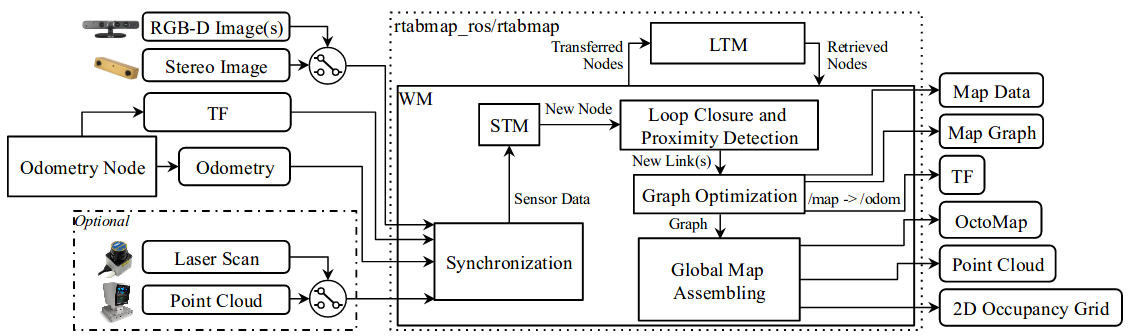
\includegraphics[scale=0.4]{img/rtabmap_scheme.png}
		\caption{Общая схема алгоритма RTAB-Map}
		\label{figurertabmap}
	\end{figure}
	
	Для одометрии по кадрам вычисляются особые точки с помощью детектора BRIEF \cite{calonder2010brief}. По сопоставлению особых точек на текущем и ключевом кадрах с помощью алгоритма PnP RANSAC \cite{brachmann2017dsac} вычисляется перемещение камеры. Полученное положение камеры корректируется с помощью алгоритма Local Bundle Adjustment \cite{zhang2006incremental} и предсказаний на основе предыдущих движений камеры. Новый ключевой кадр добавляется, когда у текущего кадра и ключевого будет мало сопоставлений. Схема вычисления одометрии представлена на рисунке \ref{figurergbdodometry}.
	
	\begin{figure}
		\centering
		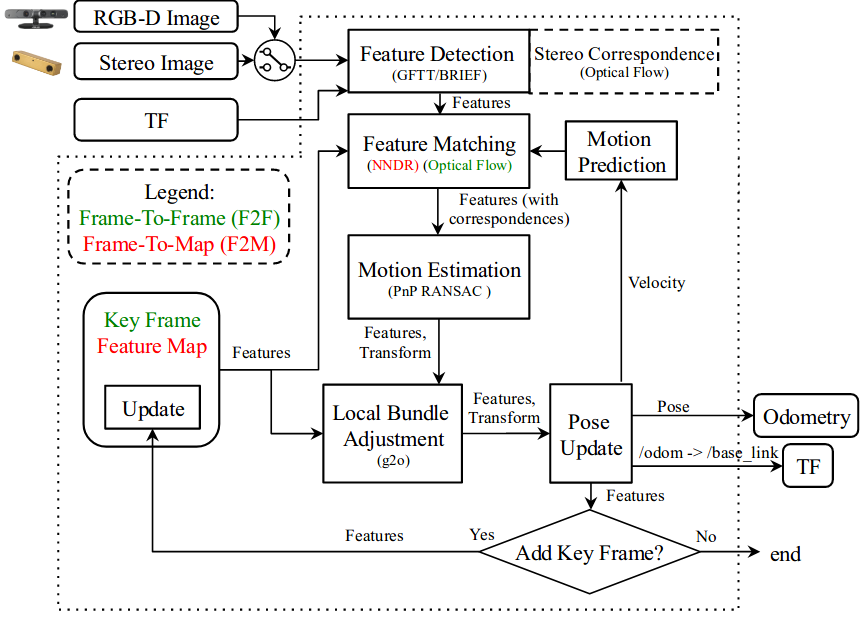
\includegraphics[scale=0.4]{img/rgbd_odometry.png}
		\caption{Схема вычисления одометрии в методе RTAB-Map}
		\label{figurergbdodometry}
	\end{figure}
	
	Картирование выполняется по локальным сеткам заполненности (occupancy grid), полученных из карт глубины. Локальные карты с помощью воксельного фильтра сшиваются в глобальную карту. При замыкании цикла карта перестраивается. Схема процесса построения карты по локальным облакам точек представлена на рисунке \ref{figuremapping}.
	
	\begin{figure}
		\centering
		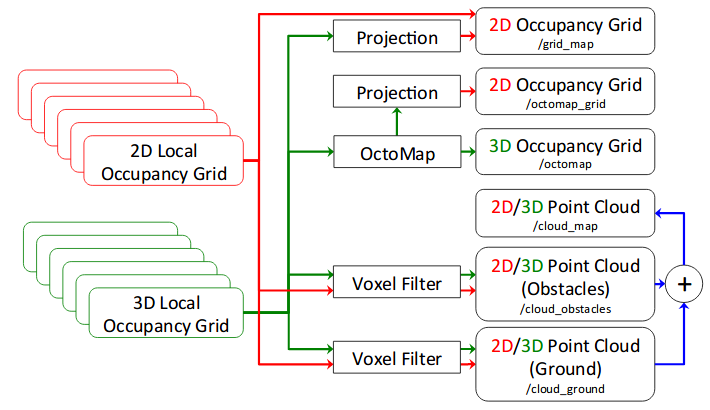
\includegraphics[scale=0.5]{img/rtabmap_mapping.png}
		\caption{Схема построения плотной глобальной карты по локальным сеткам}
		\label{figuremapping}
	\end{figure}
	
	Замыкание циклов основывается на сопоставлении особых точек на кадрах с видеопотока. Ключевая особенность данного метода - эффективное хранение изображений в памяти. Кадры хранятся в памяти как набор дескрипторов особых точек, организованный в kd-деревья. Дескрипторы извлекаются с помощью алгоритма SURF \cite{bay2006surf}. Алгоритм использует три вида памяти: WM (рабочая), в которой хранятся самые “полезные” кадры, STM (кратковременная), в которой хранятся последние кадры, и LTM (долгосрочная), в которой хранятся все кадры. Из STM в WM перемещаются те кадры, у которых больше всего похожих особых точек (похожесть мерится по дескрипторам). Для замыкания циклов используется кадр из рабочей памяти, который наиболее вероятно похож на текущий. Вероятности высчитываются байесовским фильтром. Схема процесса замыкания циклов представлена на рисунке \ref{figureloopclosing}.
	
	\begin{figure}
		\centering
		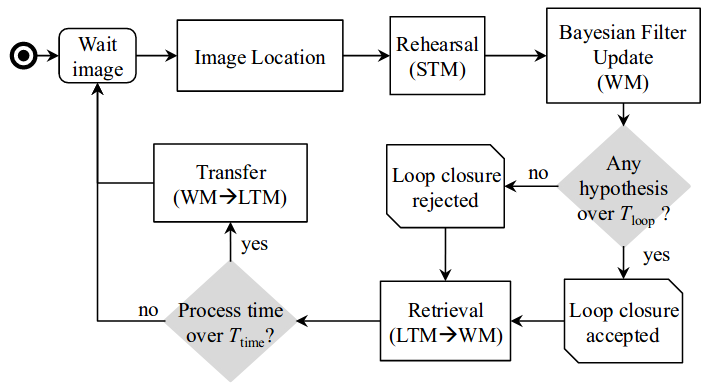
\includegraphics[scale=0.5]{img/rtabmap_loopclosure.png}
		\caption{Схема замыкания циклов в алгоритме RTAB-Map}
		\label{figureloopclosing}
	\end{figure}
	
	Данный алгоритм имеет следующие преимущества в сравнении с другими методами SLAM:
	\begin{enumerate}
		\item {Эффективная обработка данных с видеокамер и датчиков глубины в реальном времени}
		\item {Эффективное замыкание циклов}
		\item {Возможность работы в больших картах благодаря хранению долгосрочной памяти на жестком диске}
		\item {Высокая плотность построенной карты и возможность построения карты препятствий в формате Octomap}
		\item {Легкость использования в различных приложениях, а также большое количество настраиваемых параметров}
	\end{enumerate}
	Помимо преимуществ, алгоритм RTAB-Map обладает существенными недостатками:
	\begin{enumerate}
		\item {Невозможность работы в монокулярном режиме}
		\item {Потеря одометрии при отсутствии сопоставленных ориентиров}
		\item {Высокая ресурсоемкость из-за необходимости обработки трехмерных облаков точек и построения плотной карты}
	\end{enumerate}
	
	\subsection{RGBD-SLAM}
	
	Про RGBDSLAM подробно. Примеры, что он работает хуже RTABMAP'a (веер коридоров).
	
	\section{Нейросетевые методы}
	
	ANM и другие методы.
	
	%-----------------------------------------------------------------------------------------------------------------------
	% AUXILIARY TASKS
	%-----------------------------------------------------------------------------------------------------------------------
	
	\chapter{Вспомогательные задачи для vSLAM}
	
	\section{Восстановление глубины по видеопотоку}
	
	\subsection{Восстановление глубины по одиночным изображениям}
	
	Методы single-image depth estimation (fastdepth и другие s-o-t-a). Указать, что важно не только качество по RMSE, но и четкость контуров и т.д.
	
	\subsection{Восстановление глубины с использованием информации о перемещении между кадрами}
	
	Тут про рекуррентные сетки, сетки оптического потока и т.д.
	
	%------------------------------------------------------------------------------------------------------------------------------
	% OUR SLAM
	%------------------------------------------------------------------------------------------------------------------------------
	
	\chapter{Одновременное картирование и локализация с использованием вспомогательных методов}
	
	\section{Описание метода}
	
	Описание нашего слама - сетка глубины и ртабмап.
	
	\section{Программная реализация}
	
	Тут про ROS, TensorRT, сетку и ноды запуска.
	
	\section{Эксперименты}
	
	\subsection{Эксперименты в симуляторе}
	\label{section_experiments}
	
	Описание экспериментов на датасете MAOMaps.
	
	\subsection{Эксперименты на реальном роботе}
	
	Описание экспериментов на живом роботе (МПРМ или Хаски).
	
	\section{Выводы}
	
	Выводы о работе нашего слама.
	
	%--------------------------------------------------------------------------------------------------------------------------
	% EXPLORATION
	%--------------------------------------------------------------------------------------------------------------------------
	
	\chapter{Применение в задаче исследования неизвестной местности}
	
	\section{Описание задачи исследования неизвестной местности}
	
	\subsection{Постановка задачи}
	
	Постановка задачи эксплорейшена.
	
	\subsection{Метрики качества}
	
	Метрики качества эксплорейшена - покрытая за n секунд площадь и т.д.
	
	\section{Описание метода}
	
	Описание нашего фронтьерного эксплорейшена.
	
	\section{Эксперименты}
	
	Описание экспериментов на Gibson.
	
	\section{Выводы}
	
	Выводы о качестве и стабильности работы эксплорейшена.
	
	%----------------------------------------------------------------------------------------------------------------------
	% CONCLUSION
	%----------------------------------------------------------------------------------------------------------------------
	
	\chapter{Заключение}
	
	Заключение.
	
	\printbibliography
\end{document}